\definecolor{acmBlue}{HTML}{4477AA}
\definecolor{acmTeal}{HTML}{228833}
\definecolor{acmSand}{HTML}{EE7733}
\definecolor{acmGray}{HTML}{8A8F99}
\definecolor{acmGrid}{HTML}{D9DDE2}
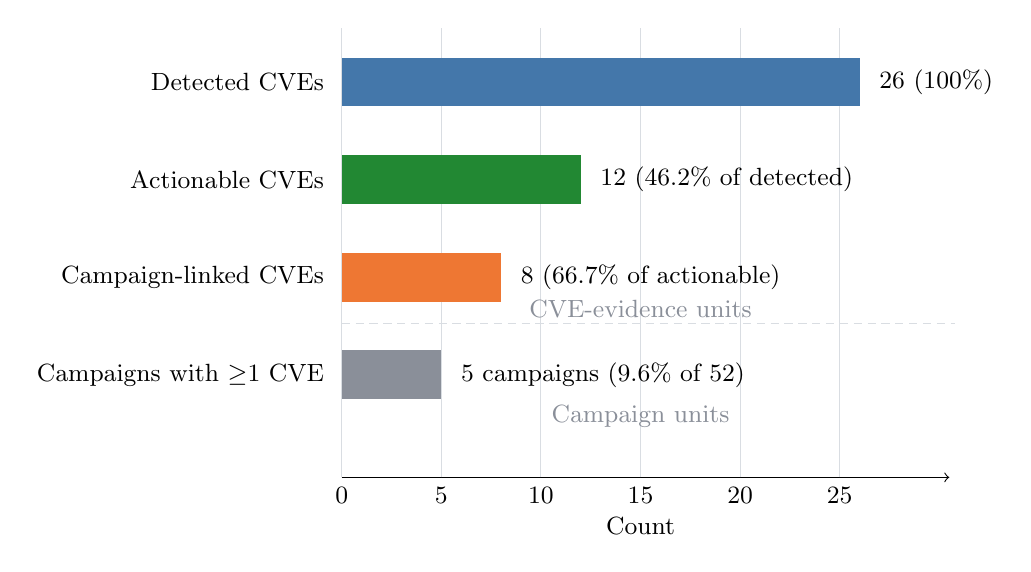
\begin{tikzpicture}[x=0.253cm,y=0.62cm,font=\small]

  % Axis
  \draw[->] (0,0) -- (30.5,0);

  \foreach \x in {0,5,10,15,20,25} {
    \draw[acmGrid] (\x,0) -- (\x,9.2);
    \node[below] at (\x,0) {\x};
  }

  \node[font=\small] at (15.0,-1.0) {Count};

  % Category labels
  \node[anchor=east] at (-0.4,8.1) {Detected CVEs};
  \node[anchor=east] at (-0.4,6.1) {Actionable CVEs};
  \node[anchor=east] at (-0.4,4.1) {Campaign-linked CVEs};
  \node[anchor=east] at (-0.4,2.1) {Campaigns with $\geq$1 CVE};

  % Bars
  \fill[acmBlue] (0,7.6) rectangle (26,8.6);
  \fill[acmTeal] (0,5.6) rectangle (12,6.6);
  \fill[acmSand] (0,3.6) rectangle (8,4.6);
  \fill[acmGray] (0,1.6) rectangle (5,2.6);

  % Divider
  \draw[densely dashed,acmGrid] (0,3.15) -- (30.8,3.15);

  % Region labels
  \node[font=\small,text=acmGray] at (15.0,3.45)
    {CVE-evidence units};

  \node[font=\small,text=acmGray] at (15.0,1.25)
    {Campaign units};

  % Values
  \node[anchor=west] at (26.5,8.1) {26 (100\%)};
  \node[anchor=west] at (12.5,6.1) {12 (46.2\% of detected)};
  \node[anchor=west] at (8.5,4.1) {8 (66.7\% of actionable)};
  \node[anchor=west] at (5.5,2.1) {5 campaigns (9.6\% of 52)};

\end{tikzpicture}
